\documentclass[11pt,a4paper]{article}

\usepackage[utf8]{inputenc}
\usepackage[margin=1in]{geometry}
\usepackage{amsmath,amssymb,amsfonts}
\usepackage{booktabs}
\usepackage{graphicx}
\usepackage{hyperref}
\usepackage{cite}
\usepackage{microtype}
\usepackage{listings}
\usepackage{xcolor}
\usepackage{tikz}
\usetikzlibrary{shapes.geometric, arrows, positioning}

\hypersetup{
    colorlinks=true,
    linkcolor=blue!70!black,
    citecolor=red!70!black,
    urlcolor=blue!60!black
}

\lstset{
    basicstyle=\ttfamily\small,
    breaklines=true,
    frame=single,
    backgroundcolor=\color{gray!10},
    keywordstyle=\color{blue!80!black}\bfseries
}

\title{\textbf{Open-SDD: Executable Architecture, Zero-Trust Harnessing, and Living Specifications for Enterprise Agentic Software Engineering}}

\author{
    \textbf{Mario Alejandro Ramos}\thanks{Computer Engineer specialising in Spatial Computing \& Agentic Architectures, NTT DATA. Email: \texttt{mario.ramos@nttdata.com}}
    \and
    \textbf{Open-SDD Research \& Architecture Initiative}
}

\date{September 2026 (Preprint)}

\begin{document}

\maketitle

\begin{abstract}
As generative artificial intelligence transitions from assistive auto-completion to multi-agent autonomous swarms, enterprise and real-world software engineering confronts an acute governance crisis: stochastic model capacity drastically outpaces deterministic verification. Uncontrolled agentic pipelines routinely amplify write throughput while severely degrading system cohesion, multiplying code duplication and accumulating latent architectural debt. 

This paper introduces \textbf{Open-SDD}, an open, model-agnostic, zero-trust specification-driven reference harness and methodological toolkit. Grounded in the fifth generation of software abstraction where architectural intent becomes an executable control plane (\textit{SpecOps}), Open-SDD formalizes a four-phase closed-loop cycle: \textit{propose $\rightarrow$ act $\rightarrow$ verify $\rightarrow$ learn}. By deprecating fragmented heuristics and eradicating legacy branded wrappers in favor of unified \texttt{sdd-*} protocols and \texttt{.sdd/} living trees, Open-SDD introduces five structural innovations: 
(i) a \textbf{Documentary Triad} operating under EARS syntax and persistent Git-native provenance; 
(ii) a \textbf{Strict Git Mode and SpecOps Lifecycle} establishing immutable phase gates, automated branch management, and a zero-tolerance \textit{Gate 0} blocking implementation without human-approved specifications; 
(iii) an \textbf{Adaptive Contextual Decision Engine} (PASS/WARN/ASK/BLOCK) mitigating the empirical \textit{Bypass Conjecture} ($E_{\text{ef}} = E_{\text{nom}}(1 - d(\phi))$) to prevent compliance disabling under false-positive fatigue; 
(iv) an \textbf{Enterprise Agentic Quality Engineering (Agentic QE)} validation substrate operating under the PACTS methodology (Proactive, Autonomous, Collaborative, Targeted, Structured) via Model Context Protocol (MCP) fleets and metamorphic invariants; 
(v) a \textbf{Universal Brownfield Modernization Spectrum} spanning from solo developers and startups to hyperscaler cloud environments (AWS, GCP, Azure) via code-first reverse engineering (\texttt{/sdd-getspecs}), Michael Feathers' Golden Characterization locks, and Martin Fowler's Strangler Fig pattern; and 
(vi) native alignment with emergent regulatory frameworks including the EU AI Act (Articles 11--15), NIST AI RMF, and ISO/IEC 42001. We demonstrate how Open-SDD relocates human authority to intent, ethics, and boundary-setting while transforming code into an ephemeral, regenerable commodity.
\end{abstract}

\noindent\textbf{Keywords:} Spec-Driven Development, Agentic Software Engineering, Zero-Trust Architecture, Living Specifications, Universal Brownfield Modernization, Agentic QE, Strict Git Mode, Human-in-the-Loop, AI Governance.

---

\section{Introduction: The Inflection Point of 2026}

Three years into the widespread deployment of Large Language Model (LLM) coding assistants, empirical data reveals a striking divergence between perceived acceleration and objective delivery stability. Randomized controlled trials by METR demonstrated that experienced engineers operating AI assistants without formal constraints were up to 19\% slower on mature codebases despite self-reporting a 20\% speed improvement \cite{metr2025}. Longitudinal source-code evaluations across 211 million lines by GitClear revealed a fourfold multiplication in duplicated code blocks and a decline of refactoring below 10\% of total change volume \cite{gitclear2025}. Similarly, DORA empirical telemetry confirmed that for every 25 percentage-point increase in ungoverned AI adoption, delivery stability suffered a 7.2\% degradation \cite{dora2024}.

The diagnostic conclusion is unambiguous: \textbf{the bottleneck in enterprise agentic engineering is not generative capability, but the absence of a deterministic control plane surrounding a stochastic process.} When left uninstrumented, autonomous agents create state coupling across interdependent components, lack transactional wave atomicity, and suffer from algorithmic collusion when generating and reviewing code within shared context windows.

To solve this dilemma, we present \textbf{Open-SDD}, an enterprise-grade, model-agnostic reference harness that transforms architectural specifications from passive, perishable documentation into executable, auditable, and enforceable reality. Open-SDD repudiates proprietary platform lock-in and vendor prefixes (eradicating all historical \texttt{kiro-*} baggage), replacing them with an open standard rooted in Git primitives, EARS syntax, and deterministic validation gates across 8 leading agent platforms.

\section{Theoretical Foundations: The Fifth Generation of Abstraction}

As articulated in recent architectural literature from Red Hat's Office of the CTO \cite{griffin2026spec}, software engineering history is defined by progressive abstraction leaps:
\begin{enumerate}
    \item \textbf{1st Generation}: Machine code (direct binary manipulation).
    \item \textbf{2nd Generation}: Assembly mnemonics (symbolic processor operations).
    \item \textbf{3rd Generation}: High-level compiled languages ($C$, Fortran, Java) masking platform instructions.
    \item \textbf{4th Generation}: Managed memory and dynamic runtimes (garbage collection, virtual machines, declarative infrastructure).
    \item \textbf{5th Generation (SDD)}: Declarative natural and structured intent as the primary executable control surface (\textit{Spec-Driven Development}).
\end{enumerate}

In this paradigm shift, code ceases to be the canonical source of truth. As illustrated in Table~\ref{tab:inversion}, SDD enacts a fundamental architectural inversion. Implementation code becomes disposable and regenerable on demand---\textit{Ambient Code}---while the specification repository hosted natively in Git governs the runtime invariant.

\begin{table}[h!]
\centering
\small
\caption{Architectural Inversion: Classical vs. Open-SDD Model (adapted from \cite{griffin2026spec}).}
\label{tab:inversion}
\resizebox{\linewidth}{!}{%
\begin{tabular}{@{}lll@{}}
\toprule
\textbf{Dimension} & \textbf{Classical Model (Legacy)} & \textbf{Open-SDD Model} \\ \midrule
Source of Truth & Source code defines behavior & Executable specifications define behavior \\
Role of Architecture & Advisory (dormant diagrams in wikis) & Enforceable, executable, and binding \\
Code Lifecycle & Primary long-term enterprise asset & Ambient code: disposable, reproducible \\
Drift Detection & Forensic post-facto (production bugs) & Pre-runtime prevention via continuous gates \\
Runtime Nature & Emergent and unpredictable & Architecturally deterministic \\
Human Oversight & Forensic code review line-by-line & High-level intent, policy, and boundary gating \\ \bottomrule
\end{tabular}%
}
\end{table}

\section{The Core Architecture: The Propose--Act--Verify--Learn Loop}

Open-SDD rejects unconstrained "vibe coding" by encapsulating agent workflows in a closed cybernetic loop:
\begin{equation}
    \text{Loop} = \langle \text{Propose} \longrightarrow \text{Act} \longrightarrow \text{Verify} \longrightarrow \text{Learn} \rangle
\end{equation}
The underlying philosophical principle states: \textit{the model proposes, the harness disposes}.

\begin{figure}[htbp]
\centering
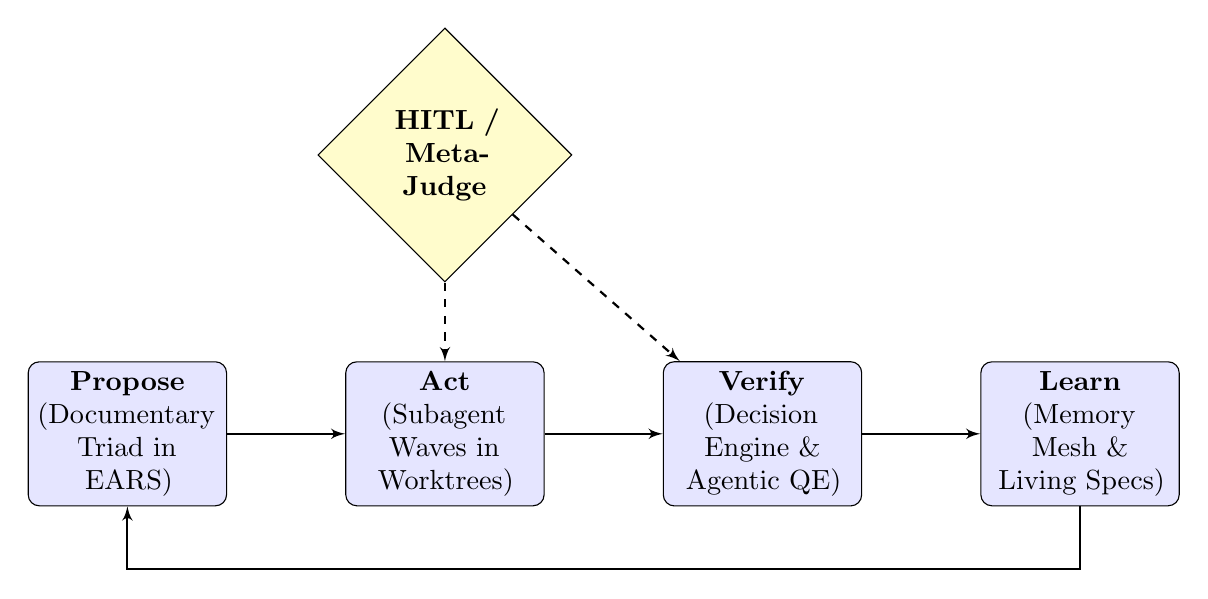
\begin{tikzpicture}[node distance=1.8cm, auto]
    \tikzstyle{block} = [rectangle, draw, fill=blue!10, text width=6.5em, text centered, rounded corners, minimum height=3em]
    \tikzstyle{judge} = [diamond, draw, fill=yellow!20, text width=4.5em, text centered, minimum height=3em]
    \tikzstyle{line} = [draw, -latex', thick]

    \node [block] (propose) {\textbf{Propose}\\ (Documentary Triad in EARS)};
    \node [block, right=1.5cm of propose] (act) {\textbf{Act}\\ (Subagent Waves in Worktrees)};
    \node [block, right=1.5cm of act] (verify) {\textbf{Verify}\\ (Decision Engine \& Agentic QE)};
    \node [block, right=1.5cm of verify] (learn) {\textbf{Learn}\\ (Memory Mesh \& Living Specs)};
    \node [judge, above=1cm of act] (judge) {\textbf{HITL / Meta-Judge}};

    \path [line] (propose) -- (act);
    \path [line] (act) -- (verify);
    \path [line] (verify) -- (learn);
    \path [line] (learn.south) -- ++(0,-0.8) -| (propose.south);
    \path [line, dashed] (judge) -- (act);
    \path [line, dashed] (judge) -- (verify);
\end{tikzpicture}
\caption{The Open-SDD cybernetic control envelope with Meta-Judge, HITL oversight, and Agentic QE validation.}
\label{fig:loop}
\end{figure}

\subsection{1. Propose: The Documentary Triad}
No generation proceeds without a bounded specification structured into three synchronized artifacts stored in \texttt{.sdd/specs/<feature>/}:
\begin{itemize}
    \item \texttt{requirements.md}: Expressed strictly in \textbf{EARS} (Easy Approach to Requirements Syntax) \cite{mavin2009ears}. All acceptance criteria must follow ubiquitous, event-driven, state-driven, or unwanted behavior patterns (e.g., \textit{WHEN [event] THEN the system SHALL [action] WHERE [constraint]}).
    \item \texttt{design.md}: Component topologies, schemas, interface contracts, and immutable \textbf{Architecture Decision Records (ADRs)}.
    \item \texttt{tasks.md}: Directed Acyclic Graphs (DAG) organizing atomic, test-driven execution waves with explicit dependency annotations (\texttt{\_Depends:\_}, \texttt{\_Boundary:\_}).
\end{itemize}

\subsection{2. Act: Transactional Worktrees and Subagent Roles}
To prevent mutable state races, each task executes within an isolated Git worktree on an ephemeral wave branch. Parallel tasks share no dirty filesystem. If a sub-task fails its acceptance criteria, its worktree is discarded; the primary repository state remains untainted by construction. Rollback ceases to be a manual emergency procedure and becomes the automatic abandonment of an unmerged branch.

\subsection{3. Verify: The Bypass Conjecture and Contextual Decision Engine}
A central theoretical finding of Ramos \cite{ramos2026zero} is that rigid binary gating induces governance self-destruction:
\begin{equation}
    E_{\text{ef}}(\phi) = E_{\text{nom}}(\phi)\cdot \bigl(1 - d(\phi)\bigr)
\end{equation}
where $E_{\text{nom}}$ is the nominal enforcement rate, $\phi$ is the false-positive rate, and $d(\phi)$ is the human-induced disablement probability. When a harness raises false alarms on harmless representations (e.g., flagging \texttt{rm -rf} within a test fixture or cleaning up a mock sandbox), developers predictably export bypass variables (e.g., \texttt{BYPASS=1}), driving real security $E_{\text{ef}} \to 0$.

Open-SDD resolves this through a 6-dimensional \textbf{Contextual Decision Engine} (evaluating phase, environment, surface, artifact type, model confidence, and risk score) producing four graduated verdicts:
\begin{itemize}
    \item \textbf{PASS}: Benign representations confirmed in non-executable fixtures or documentation.
    \item \textbf{WARN}: Acceptable process debt recorded in the audit trail without pipeline termination.
    \item \textbf{ASK}: Ambiguous boundary detection requiring Human-in-the-Loop (HITL) approval via single-use, hash-bound digital receipts.
    \item \textbf{BLOCK}: Unconditional halt reserved for confirmed critical execution risks (e.g., unverified destructive shell commands, live credential exfiltration).
\end{itemize}

\subsection{Enterprise Validation: Autonomous Quality Engineering (Agentic QE) and PACTS}
While classical software quality assurance relies on static test suites and manual post-facto assertions, enterprise SDD requires continuous, autonomous validation capable of keeping pace with high-throughput multi-agent code generation. To address this, Open-SDD integrates the \textbf{Agentic QE Framework} \cite{spiridonov2026agentic}, transitioning quality assurance from an isolated, downstream activity into an autonomous, orchestrating substrate.

Under this paradigm, quality validation is governed by the \textbf{PACTS} methodology \cite{spiridonov2026agentic,cohen2025pact}:
\begin{itemize}
    \item \textbf{Proactive}: Defect anticipation and regression risk modeling prior to commit, preventing invariant violations before state transitions occur.
    \item \textbf{Autonomous}: Decentralized QE agents automatically generate metamorphic test cases, property-based invariants, and characterization suites for legacy brownfield monoliths without requiring manual test scripting. Formally, for any invariant relation $R$ over input space $\mathcal{D}$, the QE agent verifies:
    \begin{equation}
        \forall x, x' \in \mathcal{D}, \quad R(x, x') \implies R\bigl(\mathcal{F}_{\text{legacy}}(x), \mathcal{F}_{\text{modernized}}(x')\bigr)
    \end{equation}
    \item \textbf{Collaborative}: Peer co-orchestration where autonomous QE agents challenge developer subagents through adversarial verification (\texttt{sdd-review}) under human architectural governance.
    \item \textbf{Targeted}: Dynamic scoping where test generation and execution are strictly bounded to the topological blast radius ($\text{Boundary}(T_i)$) specified in \texttt{tasks.md} and \texttt{design.md}.
    \item \textbf{Structured}: Deterministic observability and structured quality telemetry that output machine-verifiable evidence matrices into \texttt{sdd-audit}, prioritizing verifiable empirical confidence over model trust.
\end{itemize}

\subsection{4. Learn: Memory Mesh and Anti-Poisoning Quarantine}
Knowledge gained during development is partitioned into a dual-memory system:
\begin{itemize}
    \item \textbf{Session/Temporal Memory} (\texttt{.sdd/memory/session/}): Compressed ledgers retaining transient decisions and pruned logs to comply with token budget constraints.
    \item \textbf{Structural Knowledge Graph} (\texttt{.sdd/memory/graph/}): A repository-wide index mapping symbols, imports, and AST blast radii (\textit{Graph before Grep}).
    \item \textbf{Anti-Poisoning Quarantine}: Prevents indirect prompt injection by demanding that lessons captured upon gate failures pass a temperature-zero curator screening and cryptographic provenance signature before promotion to permanent steering.
\end{itemize}

\section{Strict Git Mode \& The SpecOps Lifecycle: Spec-as-Code}

A core vulnerability in contemporary AI coding harnesses is the silent divergence between project specifications and production repositories. In Open-SDD, specifications are treated with identical rigor to production source code: \textit{Spec-as-Code}.

Under \textbf{Strict Git Mode} (\texttt{.sdd/settings/git.json}), the development lifecycle is mapped directly onto a deterministic Git state machine:
\begin{equation}
    \text{State}_{\text{Git}} = \langle \text{Init Seed} \longrightarrow \text{Feature Branch} \longrightarrow \text{Spec Lock} \longrightarrow \text{Gated Impl} \longrightarrow \text{Verified Push} \rangle
\end{equation}

\subsection{The Gate 0 Invariant}
Open-SDD enforces a strict precondition prior to any code alteration. The implementation command (\texttt{/sdd-impl}) executes an immutable pre-flight check designated as \textbf{Gate 0}:
\begin{equation}
    \text{Gate}_0(F) = 
    \begin{cases} 
        \text{AUTHORIZED}, & \text{if } \text{spec.json}.\text{phase} = \texttt{"approved"} \land \text{Approvals}(F) = \mathbf{True} \\
        \text{HALTED}, & \text{otherwise (Returns \texttt{E\_SPEC\_UNAPPROVED})}
    \end{cases}
\end{equation}
If a developer or subagent attempts to generate implementation code while \texttt{spec.json} remains in \texttt{phase: "initialized"} or unapproved draft state, the execution engine halts immediately. Implementation without an approved specification is strictly blocked by construction.

\subsection{Automated SpecOps Automation}
Upon human approval of the Documentary Triad (\texttt{requirements.md}, \texttt{design.md}, \texttt{tasks.md}), Open-SDD triggers automated Git orchestration:
\begin{enumerate}
    \item \textbf{Branch Isolation}: Switches context to an isolated branch $\texttt{feat/} \circ \text{Slug}(F)$ branched from the base branch.
    \item \textbf{Spec Lock Milestone}: Commits the approved specification bundle with a standardized milestone signature (\texttt{spec(slug): lock approved documentary triad}) and pushes to origin.
    \item \textbf{Verified Implementation Push}: Following successful task completion and Agentic QE verification (\texttt{/sdd-validate-impl}), Open-SDD commits the verified implementation, pushes the branch, and automatically drafts a pull request linking all verification evidence to the originating specification.
\end{enumerate}

\section{Karpathy Behavioral Directives Mechanized}

Informal practitioner wisdom, notably synthesized by Andrej Karpathy \cite{karpathy2025}, highlights recurring LLM failure modes: overcomplication, premature abstraction, and scope drift. Open-SDD elevates these behavioral rules into machine-enforced constraints:

\begin{table}[h!]
\centering
\small
\caption{Mechanization of Karpathy Guidelines in Open-SDD.}
\label{tab:karpathy}
\resizebox{\linewidth}{!}{%
\begin{tabular}{@{}llp{6.8cm}@{}}
\toprule
\textbf{Guideline} & \textbf{Open-SDD Mechanism} & \textbf{Operational Invariant} \\ \midrule
Think Before Coding & Discovery Phase (\texttt{sdd-discovery}) & Prohibits silent assumption; forces clarifying dialogue before spec initialization. \\
Simplicity First & Hard Gate & Forbids single-use abstractions, unrequested configurability, and excessive diffs. \\
Surgical Changes & Boundary Gate & Restricts file writes strictly to declared task boundaries; rejects "polishing" untouched code. \\
Goal-Driven Execution & Verify Gate (\texttt{sdd-verify}) & Rejects task completion without captured exit codes, passing assertions, and fresh stdout evidence. \\ \bottomrule
\end{tabular}%
}
\end{table}

\section{Universal Brownfield Modernization: From Solo Developers to Hyperscalers}

Empirical software engineering data demonstrates that \textbf{over 90\% of all real-world development occurs in brownfield environments}---codebases with existing architecture, operational constraints, and latent business logic. Greenfield development is the exception; legacy is the universal norm.

A critical design criterion for Open-SDD is that \textbf{brownfield modernization is not restricted to heavy enterprise bureaucracy}. Open-SDD formalizes a scalable, multi-tier spectrum that adapts dynamically to organizational scale while preserving behavioral correctness.

\subsection{The Four-Tier Brownfield Spectrum}

\begin{table}[h!]
\centering
\caption{The Open-SDD Universal Brownfield Spectrum across Organizational Scales.}
\label{tab:brownfield-spectrum}
\resizebox{\linewidth}{!}{%
\begin{tabular}{@{}lllll@{}}
\toprule
\textbf{Dimension} & \textbf{Tier 1: Solo / Freelance} & \textbf{Tier 2: Startup / SMB} & \textbf{Tier 3: Scale-Up / OSS} & \textbf{Tier 4: Enterprise / Hyperscaler} \\ \midrule
\textbf{Primary Goal} & Grounding \& zero amnesia & Shared memory, no debt & Boundary decoupling & Zero-Trust \& compliance \\
\textbf{Bootstrap Entry} & \texttt{/sdd-getspecs} (quick) & \texttt{/sdd-getspecs} (module) & \texttt{/sdd-getspecs} + Gap & AST Graph + Blast Matrix \\
\textbf{Test Focus} & Existing unit tests & Unit + Integration in PR & Boundary-scoped suites & Agentic QE (PACTS invariants) \\
\textbf{Approval Gate} & Fast-track (\texttt{-y}, \texttt{--auto}) & Team peer review & PR spec approval in Git & Strict Git Mode + Human Gate 0 \\
\textbf{Compliance} & None (lean) & PR and changelog trails & ADR decision logs & \texttt{sdd-audit} (EU AI Act, NIST) \\
\textbf{Migration Pattern} & In-place surgical refactor & Feature-flagged service & Strangler Fig proxy & Multi-Cloud Canary / Mirroring \\ \bottomrule
\end{tabular}%
}
\end{table}

\begin{itemize}
    \item \textbf{Tier 1: Solo Developers \& Freelancers (\textit{Frictionless Brownfield})}: Addresses prompt amnesia and model hallucinations when returning to repositories after months. Running \texttt{/sdd-getspecs} extracts existing stack conventions into \texttt{.sdd/steering/}, ensuring subsequent commands modify existing code surgically without rewriting file trees or inventing incompatible dependencies.
    \item \textbf{Tier 2: Startups \& Small Teams (\textit{Agile Anti-Debt})}: Eliminates the "tribal knowledge" bottleneck (bus factor $= 1$). Reverse-engineering generates a living roadmap in \texttt{steering/roadmap.md}, cutting developer onboarding time from weeks to minutes while enforcing independent peer reviews via \texttt{sdd-review}.
    \item \textbf{Tier 3: Scale-Ups \& Open Source (\textit{Modular Modernization})}: Prevents monolithic coupling. Uses \texttt{/sdd-validate-gap} to calculate dependency blast radiuses before code changes. Tasks are strictly constrained to bounded seams (\texttt{\_Boundary:\_}), enabling atomic waves without merge conflicts.
    \item \textbf{Tier 4: Enterprise \& Hyperscalers (\textit{Zero-Trust Regulated Modernization})}: Designed for mission-critical core systems running on AWS, Google Cloud, and Microsoft Azure. Operates under the comprehensive 5-Layer Modernization Protocol detailed below.
\end{itemize}

\subsection{The 5-Layer Enterprise Modernization Protocol}
For high-assurance, multi-million-line legacy systems, Open-SDD enforces five sequential containment layers:
\begin{enumerate}
    \item \textbf{Layer 1: Structural Reconnaissance (\textit{Graph before Grep})}: Zero-LLM-cost AST dependency extraction (via Tree-Sitter and Language Server Protocols) maps afferent/efferent couplings into \texttt{.sdd/memory/graph/}. This generates an explicit blast radius matrix prior to token generation.
    \item \textbf{Layer 2: Golden Characterization Locking}: Rooted in Michael Feathers' seminal legacy methodology \cite{feathers2004working}, Open-SDD deploys Agentic QE to generate black-box characterization tests that freeze current observable behavior $B_0$ into Git. Any refactor that deviates from $B_0$ without explicit specification clearance trips an unconditional halt.
    \item \textbf{Layer 3: Living Spec Reverse-Engineering (\texttt{sdd-getspecs}) and Human Gate}: Ingestion generates unapproved spec seeds (\texttt{brief.md}, \texttt{spec.json} initialized with approvals unset, and empty EARS stubs). Human architects must review, calibrate business rules, and sign off before implementation is unlocked.
    \item \textbf{Layer 4: Transactional Surgical Implementation (\texttt{sdd-impl})}: Leverages Martin Fowler's Strangler Fig pattern \cite{fowler2004strangler} and ephemeral Git worktrees. New capabilities execute behind routing proxies or feature flags, isolated from production code paths.
    \item \textbf{Layer 5: Enterprise Governance \& Compliance Ledger (\texttt{sdd-audit})}: Produces immutable verification ledgers connecting every modified source line to its task ID, ADR justification, EARS requirement, and Agentic QE test evidence.
\end{enumerate}

\subsection{Hyperscaler Cloud Integration Patterns}
In cloud environments, Open-SDD integrates with native traffic steering mechanisms:
\begin{itemize}
    \item \textbf{AWS}: Application Load Balancers (ALB) with weighted target groups route canary traffic to modernized ECS/EKS microservices, while AWS VPC Traffic Mirroring verifies bit-level response equivalence against legacy services in shadow mode.
    \item \textbf{Google Cloud}: Cloud Run and Traffic Director orchestrate incremental traffic splitting ($1\% \to 10\% \to 100\%$), with Google Cloud Trace validating latency invariants.
    \item \textbf{Microsoft Azure}: Azure Front Door and Container Apps handle URL rewrite rules, while Azure Chaos Studio evaluates failure resilience under degraded dependency conditions.
\end{itemize}

\section{Auditability, Traceability, and Regulatory Compliance}

In heavily regulated environments, an untraced architectural decision is an unauthorized decision. Open-SDD incorporates a dedicated compliance audit command (\texttt{sdd-audit}) that compiles machine-readable and PDF reports answering key regulatory mandates:
\begin{itemize}
    \item \textbf{EU AI Act Compliance}: Full traceability of technical documentation (Art. 11), automatic logging of autonomous sessions (Art. 12), and quantified human oversight logs (Art. 14).
    \item \textbf{NIST AI RMF \& ISO/IEC 42001}: Continuous risk mapping and verifiable control evidence bound to git commit trailers.
    \item \textbf{Decision Genealogy}: Every deployed function links bi-directionally to its originating EARS requirement ID, ADR justification, executing agent model hash, and verifying human approver.
\end{itemize}

\section{Open Challenges and Future Research Directions}

While Open-SDD establishes a robust reference harness, several foundational challenges remain open for active investigation:
\begin{enumerate}
    \item \textbf{Dynamic Formal Verification and SMT Solvers}: Integrating theorem provers and SMT solvers (such as Z3 or Lean 4) directly into the verify gate to prove semantic equivalence between legacy code and regenerated ambient code mathematically.
    \item \textbf{Decentralized Cross-Repository Spec Federation}: Extending living specifications across heterogeneous micro-frontend and multi-repo architectures without introducing centralized bottleneck repositories.
    \item \textbf{Dynamic Token Economy Optimization}: Balancing the financial and computational cost of multi-agent autonomous testing fleets against the risk profile of individual software boundaries.
\end{enumerate}

\section{Conclusion}

Open-SDD demonstrates that autonomous software development at scale does not require larger models; it demands disciplined, deterministic harness engineering. By treating specifications as living, versioned source code in Git, formalizing universal brownfield modernization across all organizational scales, mechanizing Karpathy's surgical simplicity, and integrating autonomous Agentic QE validation, Open-SDD provides the foundational infrastructure necessary to turn stochastic agentic generation into predictable, enterprise-ready software engineering.

\bibliographystyle{plain}
\begin{thebibliography}{10}

\bibitem{metr2025}
J.~Becker, N.~Rush, E.~Barnes, and D.~Rein.
\newblock Measuring the impact of early-2025 {AI} on experienced open-source developer productivity.
\newblock {\em arXiv preprint arXiv:2507.09089}, 2025.

\bibitem{gitclear2025}
GitClear.
\newblock {AI} {C}opilot code quality: 2025 data suggests 4x growth in code clones.
\newblock {\em GitClear Research Reports}, 2025.

\bibitem{dora2024}
Google~Cloud DORA.
\newblock {\em Accelerate State of DevOps Report 2024--2025: AI Adoption and System Stability}.
\newblock Google, 2025.

\bibitem{griffin2026spec}
L.~Griffin and R.~Carroll.
\newblock Spec driven development: When architecture becomes executable.
\newblock {\em InfoQ Architecture Series}, January 2026.

\bibitem{ramos2026zero}
M.~A. Ramos.
\newblock {SDD-First} multi-agent orchestration for enterprise development: A zero-trust reference architecture for governing agentic software engineering at scale.
\newblock {\em Preprint DOI: 10.13140/RG.2.2.29185.42087}, August 2026.

\bibitem{karpathy2025}
A.~Karpathy.
\newblock Guidelines for mitigating common {LLM} coding pitfalls.
\newblock Codified in \url{https://github.com/multica-ai/andrej-karpathy-skills}, 2025--2026.

\bibitem{mavin2009ears}
A.~Mavin, P.~Wilkinson, A.~Harwood, and M.~Novak.
\newblock Easy approach to requirements syntax ({EARS}).
\newblock In {\em Proc. 17th IEEE International Requirements Engineering Conference}, 2009.

\bibitem{sampaio2025ai}
L.~Sampaio.
\newblock {\em AI-Assisted SDD: Spec-Driven Development with Gemini, Claude, and ai-sdd}.
\newblock Self-Published, 2025.

\bibitem{spiridonov2026agentic}
D.~Spiridonov.
\newblock Agentic {QE} Framework: Bridging classical testing to autonomous quality engineering.
\newblock {\em Quantum QE \& Agentic-QE.dev}, 2025--2026. \url{https://agentic-qe.dev}.

\bibitem{cohen2025pact}
R.~Cohen.
\newblock The {PACT} principles for autonomous agent governance.
\newblock {\em Agentics Foundation Whitepapers}, 2024--2025.

\bibitem{feathers2004working}
M.~Feathers.
\newblock {\em Working Effectively with Legacy Code}.
\newblock Prentice Hall, 2004.

\bibitem{fowler2004strangler}
M.~Fowler.
\newblock Strangler {F}ig application.
\newblock \url{https://martinfowler.com/bliki/StranglerFigApplication.html}, 2004--2020.

\end{thebibliography}

\end{document}
